\section{Arc}

%\subsection{Geometry}
The geometry of an arc is determined by $r_b$, $r_t$, $r_c$, and $rise$. 
\begin{equation}
\begin{aligned}
r_b & = AB = BO = BE \\
r_t & = AC = CG \\
r_c & = DE = DF = DG \\
c & = BC =BO - CO = BO - (OG - CG) =  r_b + r_t - rise \\
\end{aligned}
\end{equation}

\begin{figure}[h]
\centering
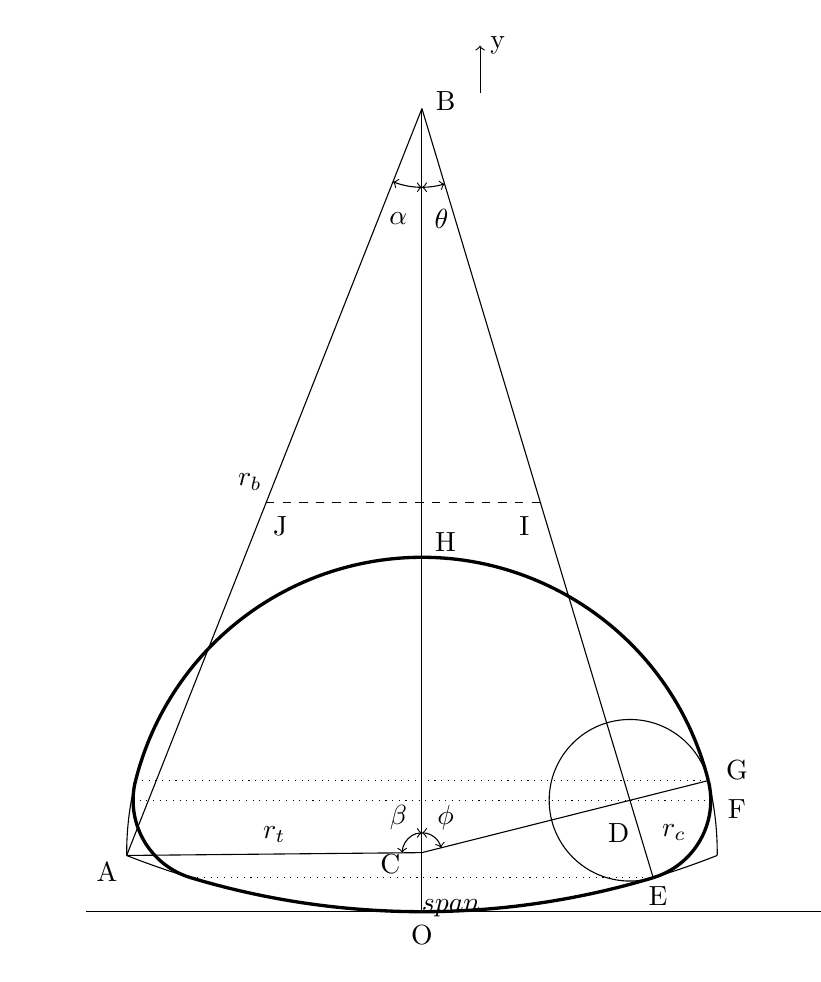
\begin{tikzpicture}

% base arc (thin) to A
\draw (-3.75, 0.714) arc[ x radius=10.2, y radius = 10.2, start angle = 248.43, end angle=291.57];
% BO
\draw (0,0) -- (0, 10.2);
% BA
\draw (0,10.2)--node[left=1]{$r_b$}(-3.75, 0.714);

\draw [<->] (0, 9.2) arc [radius=1, start angle=270, end angle=248.43];
\node at (-0.3, 8.8) {$\alpha$};

\draw [<->] (0, 9.2) arc [radius=1, start angle=270, end angle=286.74];
\node at (0.25, 8.8) {$\theta$};

% top arc (thin)
\draw (3.75, 0.714) arc[ x radius=3.75, y radius = 3.75, start angle = -0.55, end angle=180.55];
% CA
\draw (0,0.75)--node[above=0.5]{$r_t$}(-3.75, 0.714);

\draw [<->] (0, 1.0) arc [radius=0.25, start angle=90, end angle=180.55];
\node at (-0.3, 1.2) {$\beta$};

\draw [<->] (0, 1.0) arc [radius=0.25, start angle=90, end angle=14.12];
\node at (0.3, 1.2) {$\phi$};



\node at (3.2, 1.0) {$r_c$};
\node at (0, -0.3) {O};
\node at (-4.0, 0.5) {A};
\node at (0.3, 10.3) {B};
\node at (-0.4, 0.6) {C};
\node at (2.5, 1.0) {D};
\node at (3.0, 0.2) {E};
\node at (4.0, 1.3) {F};
\node at (4.0, 1.8) {G};
\node at (0.3, 4.7) {H};
\node at (1.3, 4.9) {I};
\node at (-1.8, 4.9) {J};

% IJ
\draw[dashed,thin] (-1.98,5.2) -- (1.5, 5.2);


\draw (2.642,1.415) circle [radius = 1.026];

\draw (0, 10.2) -- (2.937, 0.432);                    % BE
\draw [thin] (3.637, 1.665) -- (0,0.75);           % CG

\draw [very thick](-2.937, 0.432) arc[ x radius=10.2, y radius = 10.2, start angle = 253.26, end angle=286.74];
\draw [dotted, thin] (-2.937, 0.432) -- (2.937, 0.432);   % EE'

\draw [very thick]( 3.637, 1.665) arc[ x radius=3.75, y radius = 3.75, start angle = 14.121, end angle=165.88];
\draw[dotted, thin](-3.637, 1.665) -- (3.637, 1.665);      % GG'

\draw [very thick]( -3.637, 1.665) arc[ x radius=1.026, y radius = 1.026, start angle = 165.88, end angle=253.26];
\draw [very thick]( 3.637, 1.665) arc[ x radius=1.026, y radius = 1.026, start angle = 14.12, end angle=-73.26];
\draw[dotted, thin](-3.668, 1.415) -- (3.668, 1.415);    % FF'

\dimline [extension start length=0.2, extension end length=0.2]{(-3.668, 2.5)}{(3.668, 2.5)}{$span$}
\dimline [extension start length=0.1, extension end length=0.1]{(-5.0, 0)}{(-5.0, 4.5)}{rise}

\draw[->](-5, 0) --(4.5,0) node[below =0.5]{x} ;
\draw[->](0, 10.4) --(0,11) node[right =0.2]{y} ;

\end{tikzpicture}
\caption{Arc Section}
\label{Fig:Arc}
\end{figure}

\begin{equation}
\begin{aligned}
\cos\alpha &= \frac{r_b^2 + c^2 - r_t^2}{2r_b c} \\%= \frac{AB^2 + BC^2 - AC^2}{2 AB\times BC} \\
\cos\beta &= \frac{r_t^2 + c^2 - r_b^2}{2r_t c} \\ %= \frac{AC^2 + BC^2 - AB^2}{2 AC\times BC} \\
\cos\theta &= \frac{(r_b - r_c)^2 + c^2 - (r_t - r_c)^2}{2(r_b - r_c) c} \\ %= \frac{BD^2 + BC^2 - CD^2}{2 BD\times BC}\\
\cos\phi &= \frac{(r_t - r_c)^2 + c^2 - (r_b - r_c)^2}{2(r_t - r_c) c}  \\%= \frac{CD^2 + BC^2 - BD^2}{2 CD\times BC} \\
\end{aligned}
\end{equation}

\begin{equation}
\begin{aligned}
x_A & = r_b  \sin\alpha \\
y_A & = r_b  (1 - \cos\alpha) \\
y_B & = r_b \\
y_C & = rise - r_t = OG - CG \\
x_D &= (r_b -  r_c ) \sin\theta = (r_t - r_c) \sin \phi\\
y_D &= r_b - (r_b -  r_c ) \cos\theta = y_F \\
x_E & = r_b  \sin\theta \\
y_E & = r_b (1 - \cos\theta)\\
x_F & = x_D + r_c = span/2\\
x_G &= r_t \sin\phi \\
y_G &= y_C + r_t \cos\phi = rise - r_t (1 - \cos\phi) \\
y_H & = rise \\
\end{aligned}
\end{equation}

\begin{equation}
\begin{aligned}
A_E & =r_b^2(\theta - \sin \theta \cos \theta)  \\
P_E & =2  r_b \theta \\
T_E & = 2 r_b \sin \theta  \\
A_F & = A_E +   r_c^2 (\pi/2 - \theta) +  (x_E + x_D)(y_D-y_E)  \\
P_F & = P_E + 2  r_c (\pi/2 - \theta) \\
T_F & =  2 (x_D + r_c)  \\
A_G & = A_F +   r_c^2 (\pi/2 - \phi) +  (x_D + x_G)(y_G-y_D)   \\
P_G & = P_F + 2  r_c (\pi/2 - \phi) \\
T_G & =  2 r_t \sin \phi  \\
A_T & = A_G + r_t^2(\phi - \sin\phi\cos\phi) \\
P_T &= P_G + 2 r_t\phi
\end{aligned}
\end{equation}

\begin{figure}[h]
\centering
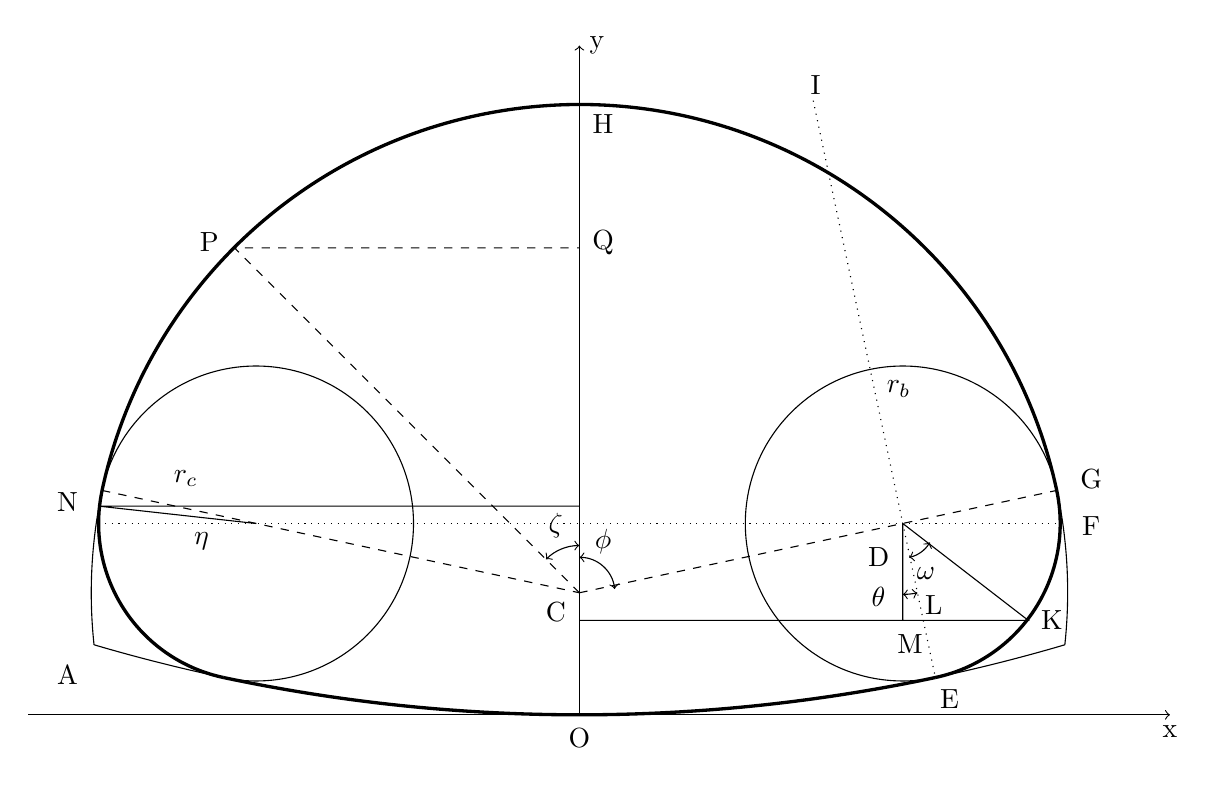
\begin{tikzpicture}

% base arc (thin) to A
\draw (-6.165, 0.890) arc[ x radius=21.8, y radius = 21.8, start angle = 253.57, end angle=286.43];
% BO
%\draw (0,0) -- (0, 21.8);

% BA
%\draw (0,21.8)--node[right=1]{$r_b$}(6.165, 0.89);

%\draw [dotted](-4.13,7.8)--node[left=1]{$r_b$}(-6.165, 0.89);  % JA

\draw [dotted](2.97,7.8)--node[right=1]{$r_b$}(4.521, 0.474);  % IE

%\draw [<->] (0, 20.8) arc [radius=1, start angle=270, end angle=286.43];
%\node at (0.2, 20.3) {$\alpha$};

%\draw [<->] (0, 20.8) arc [radius=1, start angle=270, end angle=258.03];
%\node at (-0.2, 20.3) {$\theta$};

% top arc (thin)
\draw (6.165, 0.890) arc[ x radius=6.2, y radius = 6.2, start angle = -6.11, end angle=186.11];

%\draw [dashed](0,1.55)--node[above=0.5]{$r_t$}(-6.165, 0.89); % CA

%\draw [dashed](0,1.55)--(4.521, 0.474);  % CE

\draw [dashed](0,1.55)--( 6.062, 2.850);  % CG

\draw [<->] (0, 2.0) arc [radius=0.45, start angle=90, end angle=6.11];
\node at (0.3, 2.2) {$\phi$};

%\draw [<->] (0, 2.0) arc [radius=0.45, start angle=90, end angle=192.1];
%\node at (-0.5, 2.2) {$\beta$};

\node at (-5.0, 3.0) {$r_c$};

\node at (0, -0.3) {O};
\node at (-6.5, 0.5) {A};
%\node at (0.3, 22.0) {B};
\node at (-0.3, 1.3) {C};
\node at (3.8, 2.0) {D};
\node at (4.7, 0.2) {E};
\node at (6.5, 2.4) {F};
\node at (6.5, 3.0) {G};
\node at (0.3, 7.5) {H};

\node at (3, 8) {I};
%\node at (-4, 08) {J};
\node at (6.0, 1.2) {K};
\node at (4.5, 1.4) {L};
\node at (4.2, 0.9) {M};
%\node at (0.3, 0.9) {K};
%\node at (0.3, 0.4) {L};
%\node at (6.8, 2.7) {N};

% circucle left
\draw (-4.107,2.43) circle [radius = 2.0];

%BF
%\draw (0, 21.8) -- (-4.521, 0.474);

%CG' 
\draw  [dashed](-6.062, 2.850) -- (0,1.55);

%bottom
\draw [very thick](-4.521, 0.474) arc[ x radius=21.8, y radius = 21.8, start angle = 258.03, end angle=281.97];
%top
\draw [very thick]( 6.062, 2.850) arc[ x radius=6.2, y radius = 6.2, start angle = 12.1, end angle=167.9];
%left
\draw [very thick]( -4.521, 0.474) arc[ x radius=2.0, y radius = 2.0, start angle = 258.03, end angle=167.9];
%right
\draw [very thick](  4.521, 0.474) arc[ x radius=2.0, y radius = 2.0, start angle = -78.03, end angle=12.1];

%\dimline [extension start length=0.1, extension end length=0.1]{(-7.0, 0)}{(-7.0, 7.75)}{rise}

\draw[->](-7, 0) --(7.5,0) node[below =0.5]{x} ;
\draw[->](0, 0) --(0,8.5) node[right =0.2]{y} ;

\draw(0, 1.2)--(5.7, 1.2)--(4.107,2.43) --(4.107, 1.2) ;

\draw [<->] (4.107, 1.53) arc [radius=0.9, start angle=270, end angle=281.97];
\node at (3.8, 1.5) {$\theta$};

\draw [<->] (4.187, 2.0) arc [radius=0.4, start angle=281.97, end angle=330];
\node at (4.4, 1.8) {$\omega$};

%\draw (-4.521, 0.474) --(0, 0.474);

%\draw(0, 1.2)--(-5.7, 1.2)--(-4.107,2.43) --(-4.107, 1.2) ;
%\draw [<->] (-4.107, 2.0) arc [radius=0.4, start angle=270, end angle=210];
%\node at (-4.4, 1.8) {$\omega$};
\node at (-4.8, 2.2) {$\eta$};

% circucle right
\draw (4.107,2.43) circle [radius = 2.0];

\draw[dotted](-6.107, 2.43)--(6.107, 2.43);

\draw(0, 2.65)--(-6.1, 2.65)--(-4.107,2.43);
\node at (-6.5, 2.7) {N};


\draw [dashed](0,1.55)--(-4.38, 5.93)--(0, 5.93);    % CP

\node at (-4.7, 6) {P};
\node at (0.3, 6) {Q};

\draw [<->] (0, 2.15) arc [radius=0.6, start angle=90, end angle=135];
\node at (-0.3, 2.4) {$\zeta$};


\end{tikzpicture}
\caption{Arc Section}
\label{Fig:Arc1}
\end{figure}

\noindent For $0 \le y \le y_E$, $0 \le t \le \theta$
\begin{equation}
\begin{aligned}
x & = r_b \sin t \\
y & = r_b (1 - \cos t) \\
y' & = r_b \sin t = \frac{\partial y}{\partial t}\\
A & = r_b^2(t - \sin t \cos t) \\
A' & = r_b^2(1 - \cos 2t)  = \frac{\partial A}{\partial t}\\
\frac{\partial A}{\partial y} &= 2 r_b\sin t = T_w\\
\frac{\partial}{\partial t}\left( \frac{\partial A}{\partial y}\right) &= 2 r_b\cos t \\
P & =2  r_b t\\
%T & = 2 r_b \sin t \\
\end{aligned}
\end{equation}

\noindent For $y_E \le y \le y_F$, $0 \le w \le \pi/2 - \theta $
\begin{equation}
\begin{aligned}
x &= x_D +  r_c \sin(\omega +\theta) \\
x_L &= x_D +  r_c \cos(\omega +\theta) \tan\theta \\
x'_L &= -  r_c \sin(\omega +\theta) \tan\theta \\
x''_L &=-  r_c \cos(\omega +\theta) \tan\theta \\
y &= y_D - r_c \cos(\omega +\theta) \\
y' &=  r_c \sin(\omega +\theta) \\
y'' &=  r_c \cos(\omega +\theta) \\
A &= A_E +  r_c^2 \omega - r_c^2 \sin(\omega + \theta) \cos(\omega + \theta) + r_c^2 \cos^2(\omega + \theta) \tan\theta  + (x_E +x_L) (y - y_E)  \\
A' &=  r_c^2 - r_c^2 \cos 2(\omega + \theta) - r_c^2 \sin 2(\omega + \theta) \tan\theta  + (x_E +x_L)  y' +  x'_L (y - y_E) \\
   &=  2 r_c^2 \sin^2(\omega + \theta) - 2 r_c^2 \sin(\omega + \theta) \cos(\omega + \theta)\tan\theta  + (x_E +x_L)  y' +  x'_L (y - y_E) \\
%A'' &=  2 r_c^2 \sin \left[2(\omega + \theta)\right] - 2 r_c^2 \cos [2(\omega + \theta)] \tan\theta  + (x_E +x_L)  y'' + x_L'y' +  x''_L (y - y_E) + x'_Ly'\\
\frac{\partial A}{\partial y} &= \frac{A'}{y'} = \frac{ 2 r_c^2 \sin ^2(\omega + \theta) -2 r_c^2 \sin (\omega + \theta) \cos (\omega + \theta) \tan\theta}{r_c \sin(\omega +\theta)} + x_E + x_L  - (y - y_E) \tan \theta\\
  &= 2r_c\sin(\omega + \theta) - 2r_c\cos(\omega + \theta)\tan\theta + x_E + x_D +  r_c \cos(\omega +\theta) \tan\theta \\
  & -  \left[y_D - r_c \cos(\omega +\theta) - y_E\right] \tan \theta \\
  &= 2r_c\sin(\omega + \theta) + x_E + x_D - (y_D - y_E) \tan\theta = 2x_D + 2r_c\sin(\omega + \theta) = T_w\\
\frac{\partial}{\partial \omega}\left( \frac{\partial A}{\partial y}\right) &=  2r_c\cos(\omega + \theta) \\
P &= P_E + 2 r_c \omega \\
%T &= 2 x_D + 2 r_c \sin(\omega + \theta) \\
\end{aligned}
\end{equation}

%\begin{equation}
%\begin{aligned}
%A' & =  r_c^2 - r_c^2 \cos 2(\omega + \theta) - r_c^2 \sin 2(\omega + \theta)\tan\theta + x_E y' + x_L'y + x_Ly' - x_L'y_E  \\
%A' & =  r_c^2 [1 - \cos 2(\omega + \theta) - \sin 2(\omega + \theta)\tan\theta] +  r_c(x_E + x_L) \sin (\omega + \theta) -  r_c (y - y_E) \sin(\omega + \theta)\tan\theta \\
%\end{aligned}
%\end{equation}


%where

%\begin{equation}
%\begin{aligned}
%x_K & = x_D + r_c\sin (\omega + \theta) \\ 
%y_K & = y_E + r_c [\cos\theta - \cos(\omega + \theta)] \\
%x_L  & = x_D +  (y_D - y)\tan\theta \\
%\end{aligned}
%\end{equation}


%$A_{HJF} =A_{DHF} - A_{DHI} = \frac{1}{2}r_c^2 (\omega - \theta) - \frac{1}{2}r_c^2 (\sin\omega - \sin\theta)\cos\omega$

%$FL = r_b \sin\theta$

%$KL = y_H - y_F = y - r_b (1 - \cos\theta) $

%$KI = FL - KL \tan \theta = r_b \sin\theta - [y - r_b (1 - \cos\theta)] \tan\theta$

%$A_{IKLF} =\frac{1}{2} (x_F +x_I) (y - y_F)$

%$A_H = A_F + 2A_{HJF} + 2 A_{IKLF} = A_F + r_c^2 (\omega - \theta) - r_c^2 (\sin\omega - \sin\theta)\cos\omega + (x_F +x_I) (y - y_F) $



%For $y = y_M$, $w = \frac{\pi}{2}$
%\begin{equation}
%\begin{aligned}
%A_M & = A_F + r_c^2(\frac{\pi}{2} - \theta) + (x_D + x_F)(y_D - y_F) \\
%P_M & = P_F + 2 r_c (\frac{\pi}{2} - \theta) \\
%T_M & = 2(r_b -  r_c ) \sin\theta + 2 r_c \\
%\end{aligned}
%\end{equation}

\noindent For $y_F \le y \le y_G$, $0 \le \eta \le  \pi/2-\phi$
\begin{equation}
\begin{aligned}
x & = x_D + r_c \cos\eta \\
y & = y_D + r_c \sin \eta \\
A & = A_F + r_c^2 \eta + (2x_D + r_c\cos\eta)r_c\sin\eta  \\
P & = P_F + 2 r_c \eta \\
%T & = 2 x_D + 2 r_c \cos\eta \\
y' & = r_c \cos \eta \\
%y'' & = -r_c \sin \eta \\
A' & = r_c^2 + 2x_D r_c\cos\eta + r_c^2 \cos(2\eta)  \\
%A'' & = -2x_D r_c\sin\eta - 2 r_c^2 \sin(2\eta)  \\
\frac{\partial A}{\partial y} &= \frac{A'}{y'} = \frac{ r_c^2 + 2x_D r_c\cos\eta + r_c^2 \cos(2\eta)}{r_c \cos \eta} =  2x_D + 2r_c\cos\eta = T_w \\
\frac{\partial}{\partial \eta}\left( \frac{\partial A}{\partial y}\right) & = - 2 r_c \sin \eta \\
\end{aligned}
\end{equation}

\noindent For $y_G \le y \le y_H$, $0 \le \zeta \le \phi$
\begin{equation}
\begin{aligned}
y & = y_C + r_t \cos \zeta \\
A & = A_T - r_t^2(\zeta - \sin \zeta \cos \zeta) \\
P & = P_T - 2 r_t \zeta = P_G + 2 r_t (\phi - \zeta) \\
%T & = 2r_t \sin \zeta \\
y' & = -r_t \sin \zeta \\
%y'' & = -r_t \cos \zeta \\
A' &= - r_t^2[1 - \cos(2\zeta)] \\
A'' &= -2  r_t^2 \sin(2\zeta) \\
P'(\zeta) & = -2 r_t \\
P''(\zeta) & = 0 \\
\frac{\partial A}{\partial y} &= \frac{A'}{y'} = 2 r_t \sin \zeta = T_w\\
\frac{\partial}{\partial t}\left( \frac{\partial A}{\partial y}\right) &=  2 r_t \cos \zeta\\
\end{aligned}
\end{equation}


%\begin{figure}[h]
%\centering
%\begin{tikzpicture}

% base arc (thin) to A
%\draw (-6.165, 0.890) arc[ x radius=21.8, y radius = 21.8, start angle = 253.57, end angle=286.43];
% BO
%\draw (0,0) -- (0, 21.8);
% BA
%\draw (0,21.8)--node[right=1]{$r_b$}(6.165, 0.89);

%\draw [<->] (0, 20.8) arc [radius=1, start angle=270, end angle=286.43];
%\node at (0.2, 20.3) {$\alpha$};

%\draw [<->] (0, 20.8) arc [radius=1, start angle=270, end angle=258.03];
%\node at (-0.2, 20.3) {$\theta$};

% top arc (thin)
%\draw (6.165, 0.890) arc[ x radius=6.2, y radius = 6.2, start angle = -6.11, end angle=186.11];
% CA
%\draw (0,1.55)--node[above=0.5]{$r_t$}(6.165, 0.89);

%\draw [<->] (0, 2.0) arc [radius=0.45, start angle=90, end angle=-6.11];
%\node at (0.5, 2.2) {$\beta$};

%\draw [<->] (0, 2.0) arc [radius=0.45, start angle=90, end angle=167.9];
%\node at (-0.3, 2.2) {$\phi$};

%\node at (-5.0, 3.0) {$r_c$};
%\node at (0, -0.3) {O};
%\node at (6.5, 0.5) {A};
%\node at (0.3, 22.0) {B};
%\node at (-0.5, 1.4) {C};
%\node at (0.3, 7.5) {G};
%\node at (-3.8, 2.0) {D};
%\node at (-4.7, 0.2) {E};
%\node at (-6.5, 3.0) {F};
%\node at (-6.0, 1.2) {H};
%\node at (-4.5, 1.4) {I};
%\node at (-4.2, 0.9) {J};
%\node at (0.3, 0.9) {K};
%\node at (0.3, 0.4) {L};
%\node at (-6.8, 2.7) {N};
%\node at (-6.5, 2.4) {M};
% circucle left
%\draw (-4.107,2.43) circle [radius = 2.0];

%BF
%\draw (0, 21.8) -- (-4.521, 0.474);

%CE 
%\draw  (-6.062, 2.850) -- (0,1.55);

%bottom
%\draw [very thick](-4.521, 0.474) arc[ x radius=21.8, y radius = 21.8, start angle = 258.03, end angle=281.97];
%top
%\draw [very thick]( 6.062, 2.850) arc[ x radius=6.2, y radius = 6.2, start angle = 12.1, end angle=167.9];
%left
%\draw [very thick]( -4.521, 0.474) arc[ x radius=2.0, y radius = 2.0, start angle = 258.03, end angle=167.9];
%right
%\draw [very thick](  4.521, 0.474) arc[ x radius=2.0, y radius = 2.0, start angle = -78.03, end angle=12.1];

%\dimline [extension start length=0.1, extension end length=0.1]{(-7.0, 0)}{(-7.0, 7.75)}{rise}

%\draw[->](-7, 0) --(7.5,0) node[below =0.5]{x} ;
%\draw[->](0, 22.0) --(0,22.5) node[right =0.2]{y} ;

%\draw(0, 1.2)--(-5.7, 1.2)--(-4.107,2.43) --(-4.107, 1.2) ;
%\draw [<->] (-4.107, 2.0) arc [radius=0.4, start angle=270, end angle=210];
%\node at (-4.4, 1.8) {$\omega$};

%\draw (-4.521, 0.474) --(0, 0.474);

%\draw(0, 1.2)--(-5.7, 1.2)--(-4.107,2.43) --(-4.107, 1.2) ;
%\draw [<->] (-4.107, 2.0) arc [radius=0.4, start angle=270, end angle=210];
%\node at (-4.4, 1.8) {$\omega$};

% circucle right
%\draw (4.107,2.43) circle [radius = 2.0];

%\draw(-6.107, 2.43)--(6.107, 2.43);

%\draw(0, 2.65)--(-6.1, 2.65)--(-4.107,2.43);

%\end{tikzpicture}
%\caption{Arc Section}
%\label{Fig:Arc1}
%\end{figure}

%\subsection{Calculate Maximum Discharge Using Manning's Equation}
\noindent Maximum discharge occurs close to the top of arch, the $\zeta_{max}$ is solved using Newton's method

\begin{equation}  
\zeta _{i+1} = \zeta _i - \frac{f(\zeta _i)}{f'(\zeta_i)},
\end{equation}

\noindent with %Eq. \ref{Eq:MaxQ},

\begin{equation}  
f(\zeta) = 5A'P -  2AP',
\end{equation}
and
\begin{equation}  
f'(\zeta) = 3A'P' + 5A''P - 2AP''.
\end{equation}

%\subsection{Calculate Normal Depth}
%For $Q$ less than $Q_{max}$,
%\begin{equation}  
%\alpha_{i+1} = \alpha_i -\frac{f_d(\alpha_{i})}{f'_d(\alpha_{i})}
%\end{equation}
%where
%\begin{equation}  
%f_d(\alpha_{i})= \frac{K_u}{n}A^{5/3}P^{-2/3}S^{1/2} - Q 
%\end{equation}

%\begin{equation}  
%f'_d(\alpha_{i})= \frac{K_u}{n}\left(\frac{5}{3}R^{2/3}A' -  \frac{2}{3}R^{5/3}P'\right)S^{1/2}
%\end{equation}

%\subsection{Critical Flow}
%Critical flow occurs when the specific energy of the cross-section
%\begin{equation}
%E = \frac{v^2}{2g} + y =\frac{Q^2}{2gA^2} + y 
%\end{equation}
%reaches a minimum. Namely,
%\begin{equation}
%\frac{\partial E}{\partial y} =  -\frac{Q^2}{gA^3}\frac{\partial A}{\partial y} + 1 = 0
%\end{equation}
%Newton-Raphson method is used to calculate critical depth as
%\begin{equation}  
%y_{c,i+1} = y_{c,i} -\frac{f(y_{c,i})}{f'(y_{c,i})}
%\end{equation}
%where
%\begin{equation}  
%f_c(y)= gA^3 - Q^2\frac{\partial A}{\partial y} 
%\end{equation}

%\begin{equation}  
%f'_c(y)= 3gA^2\frac{\partial A}{\partial y} - Q^2\frac{\partial ^2A}{\partial y^2} 
%\end{equation}

%\begin{equation}  
%f_c(y_{i})= 1 - \frac{Q^2}{gA^3}\frac{\partial A}{\partial y} 
%\end{equation}

%\begin{equation}  
%f'_c(y_{i})= \frac{Q^2}{gA^3} \left[ 3 \left(\frac{\partial A}{\partial y}\right)^2 - A\frac{\partial ^2 A}{\partial y^2}   \right] 
%\end{equation}

%for A and y are parameterized as a function of $t$ with $A=A(t)$, $A'=\frac{\partial A(t)} {\partial t}$, $y=y(t)$, $y'=\frac{\partial y(t)}{\partial t}$, 

%\begin{equation}  
%t_{c,i+1} = t_{c,i} -\frac{f(t_{c,i})}{f'(t_{c,i})}
%\end{equation}

%\begin{equation}  
%f_c(t)= gA^3(t) - Q^2\frac{\partial A}{\partial y}(t) 
%\end{equation}

%\begin{equation}  
%f'_c(t)= 3gA^2\frac{\partial A}{\partial t} - Q^2\frac{\partial}{\partial t}\left(\frac{\partial A}{\partial y}\right) 
%\end{equation}

%\begin{equation}  
%f_c(t)= 1 - \frac{Q^2}{gA^3}\frac{A'}{y'} 
%\end{equation}

%\begin{equation}  
%f'_c(t)= \frac{Q^2}{gA^3} \left[ 3 \left(\frac{\partial A}{\partial y}\right)^2 - A\frac{\partial ^2 A}{\partial y^2}   \right] 
%\end{equation}



